\addchapheadtotoc
\chapter{Results and Discussion}
In this chapter we introduce the experiments conducted in this work  with a discussion of the results. At first, we present the results of a Synthetic Graph Dataset created based on Stochastic Block Model (SBM), then the results of some real-world datasets (DD, Mutag,..etc).


\section{Results of Synthetic SBM Dataset}
\subsection{Stochastic Block Model SBM}
SBM is commonly known in social sciences to model group structures in friendship graph networks. As a combination of the strict block model with a stochastic element, it was able to deal with imperfect group structures and noise of real world networks. The standard SBM does not only determine the likelihood of a specific group structure belonging to a certain network. The model is based on a generative model, which enables the user to generate other network instances from a given structure or allows the prediction of missing edges \citep{SBM}.

\begin{figure}[H]
\centering
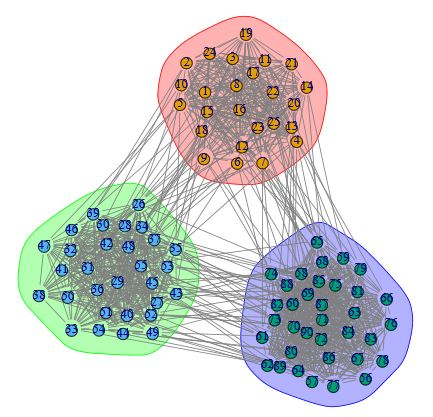
\includegraphics[scale=0.8]{LatexDiss/Dissertation/figs/SBM.JPG}
\caption[Visualization of an SBM-based graph example]{An example of a graph generated using SBM model, the graph has 90 nodes divided into three communities of size 25, 30 and 35 nodes. An edge between two nodes within the same community has a probability 0.8, while it has a probability 0.5 if the two nodes belong to different communities.}
%Source:
\label{fig:SBM_example}
\end{figure}

The basic idea of the standard SBM is that the neighborhood relations of each node only depend on the probabilities assigned to the model. Roughly speaking, the nodes are clustered in a way so that the neighbors of nodes in a group (community) have a similar neighbor pattern as well. To generate a graph $G$ of size $n$ using SBM model, the following parameters should be given: The number of communities (groups) in the graph $L$, node to community assignments ${b_1 , \ldots ,b_n}$ such that node $i$ belongs to community $b_i$, edge probability matrix $(p_{i,j})_{i,j\in\{1,\ldots, L\}}$.
Then the graph is generated by independently add an edge between any two pair of nodes $(u,v)$ with probability $p_{b_u , b_v}$.\newline
An easy thing to compute here is the average degree $d$ of each node $u$ in the graph $G=SBM(V_G, L, b_u, p_{i,j})$, which is equal to:
\begin{equation}
    d_u=\sum_{b\neq b_u} p_{b_u,b}*(\#\{v\in V_G, b_v=b \} )+p_{b_u,b_u}*(\#\{v\in V_G, b_v=b_u \}-1 )
\end{equation}
In our case and almost in every experiment, unless the opposite is mentioned, the dataset consists of 300 graphs constructed by SBM model each, each graph has $n=60$ nodes divided equally between two communities $L=2$. Other parameters ($p_{i,j}$) take different values in different graphs, and actually graphs are divided into different classes based on the corresponding values of these parameters. We consider only the case where the probabilities $p_{1,1}= p_{2,2} = p_{in}$. However,  it is obvious that  $p_{1,2}=p_{2,1}=p_{out}$ since we want an indirect graphs dataset as indicated previously.\newline
The first class of graphs corresponds to a fixed pair ($p_{in,1}, p_{out,1}$) and similarly the second one  corresponds to ($p_{in,2}, p_{out,2}$). These two pairs are always chosen so that any node in any graph in any dataset has an expected average degree equal to 10 (to preserve some difficulty in the classification problem). we refer to $r=(p_{in,1}/p_{in,2})$ by inter-classes similarity parameter, where the closer to one it is the more similar both classes are and thus the harder it is to discriminate them. 

\subsection{Graphlet Kernel results}
\begin{figure}[H]
\centering
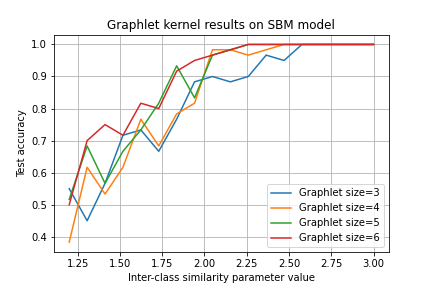
\includegraphics[scale=0.7]{LatexDiss/Dissertation/figs/graphlet_kernel_SBM_accuracy.png}
\caption[Graphlet kernel classification test accuracy as a function of Inter-classes similarity parameter]{Graphlet kernel classification test accuracy with respect to Inter-classes similarity parameter $r$. where per graph G, 2000 graphlet samples are considered to compute its graphlet spectrum vector. }
%Source:
\label{fig:graphlet_kernel_SBM}
\end{figure}

\begin{table}
\begin{center}
\begin{tabular}{|l|c|c|c|c|}
\hline
{}  &  {\sc 3-graphlets}  & {\sc 4-graphlets}  & {\sc 5-graphlets} & {\sc 6-graphlets} \\
\hline
{Computational Time (Sec)}         & 80 & 120 & 150 & 320 \\
\hline
\end{tabular}
\end{center}
\caption{Computational time per epoch of k-graphlet kernel with different k values.}
\label{table:graphlet_time}
\end{table}


\subsection{OPUs' Random Features Results}

\paragraph {Fixed inter-classes similarity and varying number of random features (Fig. \ref{fig:LightOn_adj_SBM_RF})}
\begin{figure}[H]
\centering
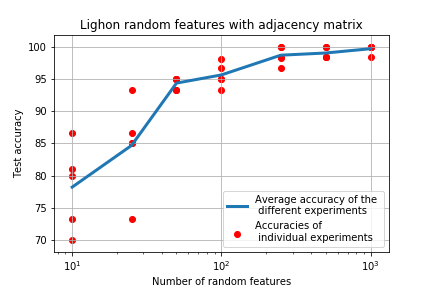
\includegraphics[scale=0.7]{LatexDiss/Dissertation/figs/LightON_adj_SBM_varying_RF.png}
\caption[Classification test accuracy as a function of the number of random features]{Classification test accuracy with respect to the number of LightOn random features. The SVM model is trained on SBM 240-sized labeled dataset. Per graph G, 2000 graphlet samples (Uniform sampling) of size 6 are considered to compute its features map $\phi(G)$. As expected, the accuracy variance drastically decrease as the number of random features increase. }
\label{fig:LightOn_adj_SBM_RF}
\end{figure}
The interesting thing here with OPUs is that the computational time does not really depend on the number of random features  as long as it is within the capacity of the OPU when we consider fixed graphlet size, in this experiment processing time was as specified in Table. \ref{table:OPU_RF_time}. 
\begin{table}[H]
\begin{center}
\begin{tabular}{|l|c|}
\hline
{\sc Computational Time (Sec)}  &  {400 Sec}\\
\hline
\end{tabular}
\end{center}
\caption{Computational time per epoch of OPUs' random features based method.}
\label{table:OPU_RF_time}
\end{table}

\paragraph{Varying inter-classes similarity and fixed number of random features (Fig. \ref{fig:LightOn_adj_SBM_mult_factor})}
The computational time in this case is presented in Table. \ref{table:OPU_multfactor_uniform_time}. We notice that there are slight differences between time values when the graphlet size change, this is due to two reasons, the first one is that OPUs' processing time does not depend on the dimension of the input nor on the number of random features as we respect its capacity, the second one is that we consider Uniform Sampling technique to sub-sample k-size graphlets, which is unlike Random Walk based sampling techniques fast and doesn't require significantly larger time when the graphlet size increases. 
\begin{figure}[H]
\centering
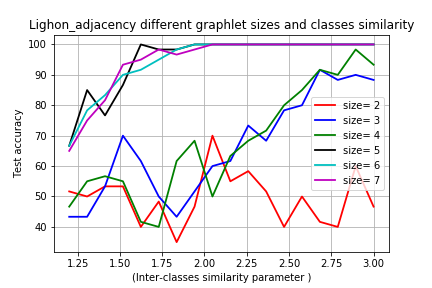
\includegraphics[scale=0.7]{LatexDiss/Dissertation/figs/LightOn_adj_SBM_Similarity_graphlet_size.png}

\caption[Classification test accuracy as a function of Inter-classes similarity parameter ]{Classification test accuracy with respect to Inter-classes similarity parameter when the number of random features is fixed to 5000 but with different sizes of the graphlet to be sampled. The SVM model is trained on SBM 240-sized labeled dataset. Per graph G, 2000 graphlet samples (Uniform sampling) of the corresponding size are considered to compute its features map $\phi(G)$.}
%Source:
\label{fig:LightOn_adj_SBM_mult_factor}
\end{figure}

\begin{table}
\begin{center}
\begin{tabular}{|l|c|c|c|}
\hline
{Graphlet Size}  &  {\sc 3} & {\sc 4}  & {\sc 5} \\
\hline
{Computational Time (Sec)}         & 630 & 720 & 810  \\
\hline
\end{tabular}
\end{center}
\caption{Computational time per epoch of OPUs' random features method using Induced Random walk}
\label{table:OPU_multfactor_IRW_time}
\end{table}


\begin{table}
\begin{center}
\begin{tabular}{|l|c|c|c|c|c|c|}
\hline
{Graphlet Size}  &  {\sc 2} & {\sc 3}  & {\sc 4}  & {\sc 5} & {\sc 6} & {7} \\
\hline
{Computational Time (Sec)}         & 340 & 357 & 362 & 378 & 400 & 412  \\
\hline
\end{tabular}
\end{center}
\caption{Computational time per epoch of OPUs' random features based method using uniform sampling technique.}
\label{table:OPU_multfactor_uniform_time}
\end{table}

\begin{figure}[H]
\centering
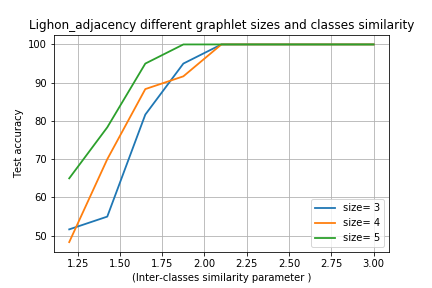
\includegraphics[scale=0.7]{LatexDiss/Dissertation/figs/LightOn_adj_SBM_similarity_graphlet_size_RW.png}
\caption[Classification test accuracy as a function of Inter-classes similarity parameter ]{Classification test accuracy with respect to Inter-classes similarity parameter when the number of random features is fixed to 5000 but with different sizes of the graphlet to be sampled. The SVM model is trained on SBM 240-sized labeled dataset. Per graph G, 2000 graphlet samples (Random Walk sampling) of the corresponding size are considered to compute its features map $\phi(G)$. This experiment is done to check if the uniform sampling technique is the reason behind the gap between accuracy curves of graphlet sizes 4 and 5 in Fig. \ref{fig:LightOn_adj_SBM_mult_factor} }
%Source:
\label{fig:LightOn_adj_SBM_multfactor_RW}
\end{figure}
However, one unexpected thing in Fig. \ref{fig:LightOn_adj_SBM_mult_factor} is that there is notably a gap between 4-graphlet and 5-graphlet curves, to detect the reason behind this gap we ran the same experiment with the same settings but using Induced Random Walk Sampling Technique , which tends to sample nodes that appear in a random walk starting from randomly chosen node (will be further explained in the report later). results are shown in Fig. \ref{fig:LightOn_adj_SBM_multfactor_RW} and the corresponding computational time is shown in Table. \ref{table:OPU_multfactor_IRW_time}.
\paragraph{Varying number of graphlet samples and fixing other parameters }
.

..

.
\subsection{Graph Convolution Network GCN}
In order to benchmark the results of Random Features-based methods with other common methods used in Graph classification, we modified and trained one of the proposed models built based on GIN (Graph Isomorphism Network), which has been reported to give brilliant results (even better than most of state-of-art classical Graph Convolutional Networks) in classifying graphs based only on their structural information in the absence of node features just like the case of our SBM dataset \citep{GCN_powerful}. 

\begin{figure}[H]
\centering
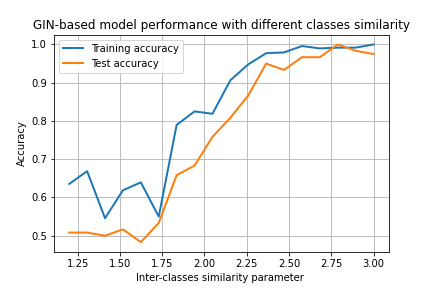
\includegraphics[scale=0.7]{LatexDiss/Dissertation/figs/GNN_GIN.png}

\caption[GCN model's classification test accuracy as a function of Inter-classes similarity parameter ]{GCN model's classification test accuracy with respect to Inter-classes similarity parameter. The  model is trained on SBM 240-sized labeled dataset.}
%Source:
\label{fig:GCN_GIN_SBM_multfactor_RW}
\end{figure}

\begin{table}
\begin{center}
\begin{tabular}{|l|c|c|c|}
\hline
{Epoch processing time (Sec)}  &  {total training time (Sec)} \\
\hline
0.29 & 87  \\
\hline
\end{tabular}
\end{center}
\caption{Computational time per epoch of the GCN GIN-based model.}
\label{table:OPU_multfactor_IRW_time}
\end{table}
The model consists of 5 GIN layers followed by two fully connected layers where the dimensions of hidden layers are equal to 4. Comparing GCN performance to the one we got using OPUs random features (Fig. \ref{fig:LightOn_adj_SBM_multfactor_RW} and Fig. \ref{fig:LightOn_adj_SBM_mult_factor}) we can say that the performance of Random Features based methods is slightly better when the graphlet size is greater than 4, especially using Induced Random Walk sampling technique. However, the training time of GCN model still notably better (I should check if I can do something with LightOn platform to enhance its time, so the report will be fixed later). 

\section{DD Real-world Data set}
\subsection{Graphlet Kernel Results}
.

.

.
\subsection{OPUs’ Random Features Results}
\begin{figure}[H]
\centering
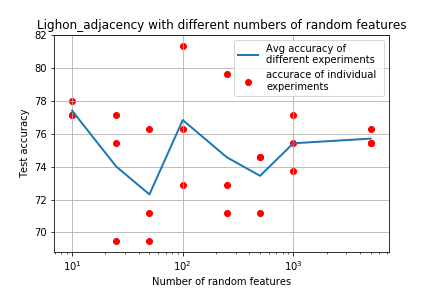
\includegraphics[scale=0.7]{LatexDiss/Dissertation/figs/LightOn_adj_DD_varying_RF.png}

\caption[Classification test accuracy as a function of the number of random features]{Classification test accuracy with respect to the number of random features on DD Dataset}
%Source:
\label{fig:LightON_DD_multfactor_RW}
\end{figure}

\subsection{Graph Convolutional Networks GCNs Results}
.

.

.